\subsubsection{Varnish}
\label{soa:tecnologias:varnish}

\gls{db:varnish} es un proxy reverso HTTP, a veces referenciado como HTTP accelerator o a \eng{web accelerator}, que almacena archivos y framentos de archivos en memoria, lo que reduce el tiempo de respuestea y el ancho de banda de red para las mismas solicitudes.\cite[p.~20]{varnish2016}

El proyecto Varnish fue iniciado por Verdens Gang en el 2005, contó con la gerencia, infraestructura y desarrollos adicionales aportados por la comunidad Noruega de Linux, que mas tarde pasó a una empresa independiente, Varnish Software.

Dependiendo de su instalación, varnish puede ser usado para:

\begin{itemize}
  \item web application firewall,
  \item DDoS attack defender,
  \item load balancer,
  \item integration point,
  \item single sign-on gateway,
  \item authentication and authorization policy mechanism,
  \item quick fix for unstable backends,
  \item HTTP router
\end{itemize}

Como mencionamos anteriormente, \gls{db:varnish} es un acelerador de aplicaciones web, que se instala delante de cualquier servidor HTTP y se configura para almacenar en la caché del servidor una copia del recurso solicitado. Pensado para mejorar el rendimiento de aplicaciones web con contenidos pesados y APIs altamente consumidas, este será nuestro caso.

para la conclusión
Para nuestra implementación, se instalará varnish delante del balanceador de carga y por lo tanto, delante de las instancias replicadas en las que se encuentran las diferentes APIs, de esta manera, los accesos recurrentes a los mismos \eng{end points}, serán obtenidos desde la cache de varnish, en lugar de llegar a cualquiera de las APIs, logrando obtener mejores tiempos de respuesta.


conseguir fuente de este dato
Actualmente es utilizado por una gran cantidad de sitios web con alta demanda de tráfico como pueden ser: The New York Times, The Guardian, The Hindu, y sitios de redes sociales y contenidos como Wikipedia, Facebook, Twitter, Vimeo, Tumblr, entre otros. De los top 10K sitios en la web, alrededor de una décima parte usan Varnish Cache.


\begin{figure}[H]
  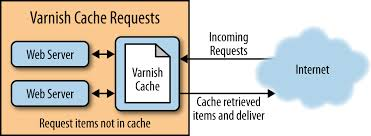
\includegraphics[width=\linewidth]{src/images/03-capitulo-3/tecnologias/varnish/reverse-proxy.jpg}
  \caption{Varnish Reverse Proxy}
  \label{fig:varnish}
\end{figure}

\paragraph{Licencia}

Varnish Cache es software libre, licenciado bajo una licencia BSD

\paragraph{Instalación}

Varnish se distribuye en los respositorios de paquetes de Ubuntu, pero puede suceder que el paquete se encuentre desactualizado por lo tanto se recomienda usar los respositorios de paquestes de varnish-cache.org.
Para usar los respositorios de varnish-cache.org e instalar Varnish en Ubuntu 14.04, debemos ejecuatar la siguiente secuencias de comandos:

\begin{listing}[H]
  \bashfile{src/03-capitulo-3/tecnologias/cache/code/varnish/00-preparacion.sh}
  \caption{Instalación de Varnish}
  \label{soa:tecnologias:varnish-cache:bash-preparacion}
\end{listing}
